\documentclass[]{tufte-handout}

% ams
\usepackage{amssymb,amsmath}

\usepackage{ifxetex,ifluatex}
\usepackage{fixltx2e} % provides \textsubscript
\ifnum 0\ifxetex 1\fi\ifluatex 1\fi=0 % if pdftex
  \usepackage[T1]{fontenc}
  \usepackage[utf8]{inputenc}
\else % if luatex or xelatex
  \makeatletter
  \@ifpackageloaded{fontspec}{}{\usepackage{fontspec}}
  \makeatother
  \defaultfontfeatures{Ligatures=TeX,Scale=MatchLowercase}
  \makeatletter
  \@ifpackageloaded{soul}{
     \renewcommand\allcapsspacing[1]{{\addfontfeature{LetterSpace=15}#1}}
     \renewcommand\smallcapsspacing[1]{{\addfontfeature{LetterSpace=10}#1}}
   }{}
  \makeatother

\fi

% graphix
\usepackage{graphicx}
\setkeys{Gin}{width=\linewidth,totalheight=\textheight,keepaspectratio}

% booktabs
\usepackage{booktabs}

% url
\usepackage{url}

% hyperref
\usepackage{hyperref}

% units.
\usepackage{units}


\setcounter{secnumdepth}{-1}

% citations
\usepackage{natbib}
\bibliographystyle{plainnat}


% pandoc syntax highlighting
\usepackage{color}
\usepackage{fancyvrb}
\newcommand{\VerbBar}{|}
\newcommand{\VERB}{\Verb[commandchars=\\\{\}]}
\DefineVerbatimEnvironment{Highlighting}{Verbatim}{commandchars=\\\{\}}
% Add ',fontsize=\small' for more characters per line
\newenvironment{Shaded}{}{}
\newcommand{\AlertTok}[1]{\textcolor[rgb]{1.00,0.00,0.00}{\textbf{#1}}}
\newcommand{\AnnotationTok}[1]{\textcolor[rgb]{0.38,0.63,0.69}{\textbf{\textit{#1}}}}
\newcommand{\AttributeTok}[1]{\textcolor[rgb]{0.49,0.56,0.16}{#1}}
\newcommand{\BaseNTok}[1]{\textcolor[rgb]{0.25,0.63,0.44}{#1}}
\newcommand{\BuiltInTok}[1]{#1}
\newcommand{\CharTok}[1]{\textcolor[rgb]{0.25,0.44,0.63}{#1}}
\newcommand{\CommentTok}[1]{\textcolor[rgb]{0.38,0.63,0.69}{\textit{#1}}}
\newcommand{\CommentVarTok}[1]{\textcolor[rgb]{0.38,0.63,0.69}{\textbf{\textit{#1}}}}
\newcommand{\ConstantTok}[1]{\textcolor[rgb]{0.53,0.00,0.00}{#1}}
\newcommand{\ControlFlowTok}[1]{\textcolor[rgb]{0.00,0.44,0.13}{\textbf{#1}}}
\newcommand{\DataTypeTok}[1]{\textcolor[rgb]{0.56,0.13,0.00}{#1}}
\newcommand{\DecValTok}[1]{\textcolor[rgb]{0.25,0.63,0.44}{#1}}
\newcommand{\DocumentationTok}[1]{\textcolor[rgb]{0.73,0.13,0.13}{\textit{#1}}}
\newcommand{\ErrorTok}[1]{\textcolor[rgb]{1.00,0.00,0.00}{\textbf{#1}}}
\newcommand{\ExtensionTok}[1]{#1}
\newcommand{\FloatTok}[1]{\textcolor[rgb]{0.25,0.63,0.44}{#1}}
\newcommand{\FunctionTok}[1]{\textcolor[rgb]{0.02,0.16,0.49}{#1}}
\newcommand{\ImportTok}[1]{#1}
\newcommand{\InformationTok}[1]{\textcolor[rgb]{0.38,0.63,0.69}{\textbf{\textit{#1}}}}
\newcommand{\KeywordTok}[1]{\textcolor[rgb]{0.00,0.44,0.13}{\textbf{#1}}}
\newcommand{\NormalTok}[1]{#1}
\newcommand{\OperatorTok}[1]{\textcolor[rgb]{0.40,0.40,0.40}{#1}}
\newcommand{\OtherTok}[1]{\textcolor[rgb]{0.00,0.44,0.13}{#1}}
\newcommand{\PreprocessorTok}[1]{\textcolor[rgb]{0.74,0.48,0.00}{#1}}
\newcommand{\RegionMarkerTok}[1]{#1}
\newcommand{\SpecialCharTok}[1]{\textcolor[rgb]{0.25,0.44,0.63}{#1}}
\newcommand{\SpecialStringTok}[1]{\textcolor[rgb]{0.73,0.40,0.53}{#1}}
\newcommand{\StringTok}[1]{\textcolor[rgb]{0.25,0.44,0.63}{#1}}
\newcommand{\VariableTok}[1]{\textcolor[rgb]{0.10,0.09,0.49}{#1}}
\newcommand{\VerbatimStringTok}[1]{\textcolor[rgb]{0.25,0.44,0.63}{#1}}
\newcommand{\WarningTok}[1]{\textcolor[rgb]{0.38,0.63,0.69}{\textbf{\textit{#1}}}}

% longtable
\usepackage{longtable,booktabs}

% multiplecol
\usepackage{multicol}

% strikeout
\usepackage[normalem]{ulem}

% morefloats
\usepackage{morefloats}


% tightlist macro required by pandoc >= 1.14
\providecommand{\tightlist}{%
  \setlength{\itemsep}{0pt}\setlength{\parskip}{0pt}}

% title / author / date
\title[分散の加法性を視覚的に理解する]{分散の加法性を視覚的に理解する}
\author{Sampo Suzuki, CC 4.0 BY-NC-SA}
\date{2021-05-30}

% --- 参考資料 ----------------------------------------------------------------
% https://github.com/Gedevan-Aleksizde/Japan.R2019/blob/master/latex/preamble.tex
% https://teastat.blogspot.com/2019/01/bookdown.html

% --- Packages ----------------------------------------------------------------
% 日本語とtufte, kableExtraを使うために必要なTeXパッケージ指定
% tufteではA4サイズの指定が不可能
%  A4 210mm x 297mm
%   \usepackage[a4paper, total={6.5in, 9.5in}]{geometry}
%   \usepackage{indentfirst}   # tinytexのリポジトリには存在しない?
% \usepackage[a4paper, total={160mm, 247mm}, left=25mm, top=25mm]{geometry}
% \usepackage[pdfbox,tombo]{gentombow}  % トンボを設定する場合は有効にする
% \usepackage{ifthen}                     % 条件分岐用 \ifthenelse{条件}{T}{F}
\usepackage{booktabs}                   % ここからkableExtra用パッケージ
\usepackage{longtable}                  % 
\usepackage{array}                      % 
\usepackage{multirow}                   % 
\usepackage{wrapfig}                    % 
\usepackage{float}                      % 
\usepackage{colortbl}                   % 
\usepackage{pdflscape}                  % 
\usepackage{tabu}                       % 
\usepackage{threeparttable}             % 
\usepackage{threeparttablex}            % 
\usepackage[normalem]{ulem}             % 
\usepackage{inputenc}                   % 
\usepackage{makecell}                   % 
\usepackage{xcolor}                     % ここまでkableExtra用
\usepackage{amsmath}                    % 
\usepackage{fontawesome5}               % fontawesomeを使うために必要
\usepackage{subfig}
\usepackage{xeCJK}                      % 以下、日本語フォント用に必要
\usepackage[noto]{zxjafont}             % Linux環境ではこちを指定
% \usepackage[haranoaji]{zxjafont}      % Windows環境ではこちらを指定する
\usepackage{zxjatype}
\usepackage{pxrubrica}                  % ルビ用
\usepackage{hyperref}                   % ハイパーリンク用必要?

% --- Index ------------------------------------------------------------------
% https://texwiki.texjp.org/?%E7%B4%A2%E5%BC%95%E4%BD%9C%E6%88%90
% これを指定するとIndex(索引)は作成されるが参照ページがズレる
% 中間ファイルの.indではページはズレていないので、その後の結合処理がおかしい
% \usepackage{makeidx}
% \makeindex
% \usepackage{showidx}                  % 索引確認用

% --- Table of Contentes ------------------------------------------------------
% TOCにLOT(List of Tables), LOF(List of Figures), Bibliography, Indexを表示
% \usepackage[nottoc]{tocbibind}

% --- Fonts -------------------------------------------------------------------
% フォントしては index.html でも可能(pandoc用オプションは index.htmlにて)
% \setCJKmonofont{Source Han Code JP}
\setmonofont{Source Han Code JP}
% \setjamonofont{Source Han Code JP}

% ## 日本語フォントの扱いについてはzxjafontパッケージの解説を参照のこと
% # https://mirror.las.iastate.edu/tex-archive/language/japanese/zxjafont/zxjafont.pdf
% #
% ## Windows環境ではなぜかNotoフォントが認識されないので源ノシリーズベースの
% ## 原ノ味フォントかIPAexフォントを利用する(原ノ味はtlmgrでインストール可)
% # \usepackage[haranoaji]{zxjafont}
% # \usepackage[ipaex]{zxjafont}
% #
% ## Windows環境でNotoフォントを指定したい場合は以下のようにheader-includeで
% ## 個別に指定する(setCJKxxxfotnの指定は必要?)
% # \setmainfont{NotoSerifCJKjp-Regular.otf}[BoldFont=NotoSerifCJKjp-Bold.otf]
% # \setsansfont{NotoSansCJKjp-Regular.otf}[BoldFont=NotoSansCJKjp-Bold.otf]
% # \setmonofont{NotoSansMonoCJKjp-Regular.otf}[BoldFont=NotoSansMonoCJKjp-Bold.otf]
% ## モノフォントは源ノ角コード(Source Code Proの日本語版)がおすゝめ
% # \setmonofont{SourceHanCodeJP-Regular.otf}[BoldFont=SourceHanCodeJPS-Bold.otf]

\begin{document}

\maketitle




\hypertarget{introduction}{%
\section{\texorpdfstring{\textbf{Introduction}}{Introduction}}\label{introduction}}

 2021年度データ分析勉強会のテキストである『統計解析のはなし』\citep{ToukeiKaisekinoHanashi}の「標本が2つになれば」(P26〜)には分散の加法性の話が出てきます。分散の加法性は理解できるようでいて、理解できていないので、\textbf{R}を使って分散の加法性を可視化しながら説明してみます。

以降、平均値\(\mu\)、標準偏差\(\sigma\)、分散\(\sigma^2\)である正規分布を\(N(\mu, \sigma^2)\)と表記します。

 

\hypertarget{ux52a0ux6cd5ux6027ux3092ux53efux8996ux5316ux3059ux308b}{%
\section{\texorpdfstring{\textbf{加法性を可視化する}}{加法性を可視化する}}\label{ux52a0ux6cd5ux6027ux3092ux53efux8996ux5316ux3059ux308b}}

 以下の平均値と標準偏差を持つ二つの正規分布を\texttt{rnorm()}関数による正規分布乱数を用いて作成\footnote{n
  = \ensuremath{5\times 10^{6}}個の値を作成しています}します。ここでは処理の都合上、二つをデータフレームにまとめてあります。

\begin{longtable}[]{@{}llll@{}}
\caption{二つの正規分布}\tabularnewline
\toprule
正規分布 & 平均 & 標準偏差 & 備考 \\
\midrule
\endfirsthead
\toprule
正規分布 & 平均 & 標準偏差 & 備考 \\
\midrule
\endhead
\(N(\mu_a, \sigma^2_a)\) & \(\mu_a = 10\) & \(\sigma_a = 10\) & \\
\(N(\mu_b, \sigma^2_b)\) & \(\mu_b = 30\) & \(\sigma_b = 10\) & \\
\bottomrule
\end{longtable}

\begin{Shaded}
\begin{Highlighting}[numbers=left,,]
\NormalTok{x }\OtherTok{\textless{}{-}} \FunctionTok{data.frame}\NormalTok{(}\AttributeTok{a =} \FunctionTok{rnorm}\NormalTok{(n, }\AttributeTok{mean =} \DecValTok{10}\NormalTok{, }\AttributeTok{sd =} \DecValTok{10}\NormalTok{),}
                \AttributeTok{b =} \FunctionTok{rnorm}\NormalTok{(n, }\AttributeTok{mean =} \DecValTok{30}\NormalTok{, }\AttributeTok{sd =} \DecValTok{10}\NormalTok{))}
\end{Highlighting}
\end{Shaded}

\begin{marginfigure}

{\centering 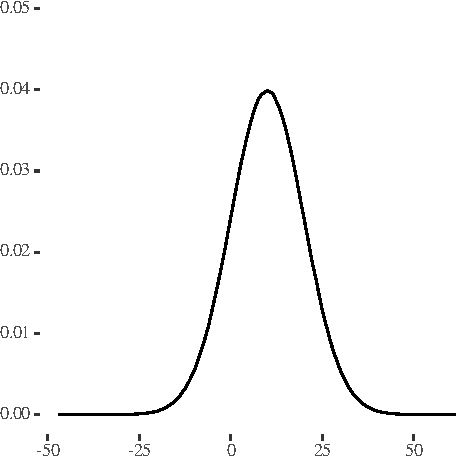
\includegraphics{AdditivityOfVariance_files/figure-latex/unnamed-chunk-2-1} 

}

\caption[$N(\mu_a, \sigma^2_a)$の分布]{$N(\mu_a, \sigma^2_a)$の分布}\label{fig:unnamed-chunk-2}
\end{marginfigure}

\begin{marginfigure}

{\centering 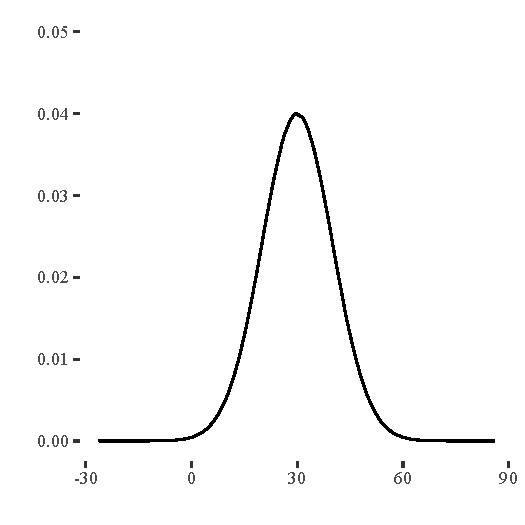
\includegraphics{AdditivityOfVariance_files/figure-latex/unnamed-chunk-3-1} 

}

\caption[$N(\mu_b, \sigma^2_bb)$の分布]{$N(\mu_b, \sigma^2_bb)$の分布}\label{fig:unnamed-chunk-3}
\end{marginfigure}

\begin{longtable}[]{@{}lccl@{}}
\caption{二つの正規分布の要約統計量}\tabularnewline
\toprule
正規分布 & 平均 & 標準偏差 & 備考 \\
\midrule
\endfirsthead
\toprule
正規分布 & 平均 & 標準偏差 & 備考 \\
\midrule
\endhead
\(N(\mu_a, \sigma^2_a)\) & 9.9951475 & 9.9959159 & \\
\(N(\mu_b, \sigma^2_b)\) & 29.9989783 & 10.0051801 & \\
\bottomrule
\end{longtable}

この二つの正規分布\(N(\mu_a, \sigma^2_a)\)と\(N(\mu_b,\sigma^2_b)\)からランダムサンプリングにより一つずづ値を取り出して加算します。すなわち
 
\[N(\mu_a, \sigma^2_a)\mbox{ から取り出した値} + N(\mu_b,\sigma^2_b)\mbox{ から取り出した値}\]

という新しい値を作成します。取り出した値は元に戻し、同様の取り出し、加算を繰り返すと以下のようなデータが作成できます。ここではスペースの都合で先頭から限定して表示しています。

\begin{Shaded}
\begin{Highlighting}[numbers=left,,]
\NormalTok{c }\OtherTok{\textless{}{-}} \FunctionTok{c}\NormalTok{(}\FunctionTok{sample}\NormalTok{(x}\SpecialCharTok{$}\NormalTok{a, n, }\AttributeTok{replace =} \ConstantTok{TRUE}\NormalTok{) }\SpecialCharTok{+} \FunctionTok{sample}\NormalTok{(x}\SpecialCharTok{$}\NormalTok{b, n, }\AttributeTok{replace =} \ConstantTok{TRUE}\NormalTok{))}
\FunctionTok{head}\NormalTok{(c, }\DecValTok{50}\NormalTok{)}
\end{Highlighting}
\end{Shaded}

\begin{verbatim}
##  [1] 57.33431 13.86405 21.24315 21.52298 60.14019 64.89915 39.53705 30.66057
##  [9] 35.58985 44.39301 42.75026 24.11251 46.36193 33.31220 35.95976 25.68859
## [17] 46.92637 70.78838 57.07144 70.56954 47.77346 31.30232 26.13623 54.24486
## [25] 33.07926 27.85359 46.79052 56.22061 44.89961 42.29841 40.51847 48.20768
## [33] 61.10274 53.15060 39.06615 45.27197 12.96846 46.94400 37.67426 49.17930
## [41] 55.30332 43.38246 37.50048 16.14157 53.31532 36.56948 36.82211 35.10256
## [49] 53.73004 39.41396
\end{verbatim}

分散の加法性により上記のデータは\(N(\mu_a + \mu_b, \sigma^2_a + \sigma^2_b))\)という正規分布になるはずですが実際はどうでしょう。各正規分布の平均値と分散を比較します。

\begin{longtable}[]{@{}lccl@{}}
\toprule
正規分布 & 平均 & 分散 & 備考 \\
\midrule
\endhead
\(N(\mu_a, \sigma^2_a)\) & 9.9951475 & 99.9183346 & 元の分布 \\
\(N(\mu_b, \sigma^2_b)\) & 29.9989783 & 100.1036293 & 元の分布 \\
\(N(\mu_a + \mu_b, \sigma^2_a + \sigma^2_b))\) & 39.9941258 &
200.0219639 & 分散の加法性 \\
\(N(\mu_c, \sigma^2_c)\) & 39.9905755 & 200.0174879 & \\
\bottomrule
\end{longtable}

このように確かに分散の加法性が成り立っており、正規分布\(N(\mu_a, \sigma^2_a)\)や\(N(\mu_b,\sigma^2_b)\)より横に広がった正規分布になっていることが分かります。

\begin{marginfigure}

{\centering 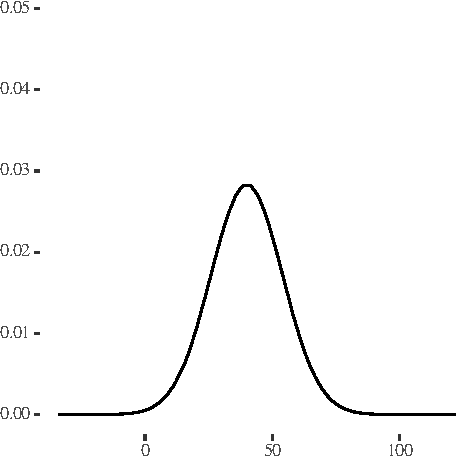
\includegraphics{AdditivityOfVariance_files/figure-latex/unnamed-chunk-5-1} 

}

\caption[$N(\mu_c, \sigma^2_c)$の分布]{$N(\mu_c, \sigma^2_c)$の分布}\label{fig:unnamed-chunk-5}
\end{marginfigure}

\newpage

\hypertarget{ux540cux4e00ux306eux6b63ux898fux5206ux5e03ux304bux3089ux53d6ux308aux51faux3057ux5024ux3092ux52a0ux7b97ux3057ux305fux5834ux5408}{%
\subsection{\texorpdfstring{\textbf{同一の正規分布から取り出し値を加算した場合}}{同一の正規分布から取り出し値を加算した場合}}\label{ux540cux4e00ux306eux6b63ux898fux5206ux5e03ux304bux3089ux53d6ux308aux51faux3057ux5024ux3092ux52a0ux7b97ux3057ux305fux5834ux5408}}

 次に二つの正規分布\(N(\mu_a, \sigma^2_a)\)と\(N(\mu_b,\sigma^2_b)\)がまったく等しいと仮定します。つまり

\[\mu_a = \mu_b = \mu_d\]

\[\sigma_a = \sigma_b = \sigma_d\]

という正規分布\(N(\mu_d, \sigma^2_d)\)を作成します。

\begin{Shaded}
\begin{Highlighting}[numbers=left,,]
\NormalTok{d }\OtherTok{\textless{}{-}} \FunctionTok{rnorm}\NormalTok{(n, }\AttributeTok{mean =} \DecValTok{10}\NormalTok{, }\AttributeTok{sd =} \DecValTok{10}\NormalTok{)}
\FunctionTok{head}\NormalTok{(d, }\DecValTok{50}\NormalTok{)}
\end{Highlighting}
\end{Shaded}

\begin{verbatim}
##  [1]  2.2233014  1.5846010  9.6193505  6.4874410 -6.7454230  3.7869663
##  [7]  7.1527368  8.8026565 15.4411933  9.4532447 32.2050733 -3.9343231
## [13] -0.5036607 16.6210855 12.6110213 16.7782865  3.2212688  2.9894326
## [19]  2.5727131 12.8557626 17.3988821 11.1802089  4.8892306 15.0641506
## [25]  5.3592454 12.9890084 20.9063492  9.4312083  9.8147737 -4.3556116
## [31] 20.9061069  0.3316442  0.5345106 17.6295992 11.4236104 -2.4654854
## [37] 14.2736619  4.6445990  7.4769036  8.6161968  7.1881268  9.9389923
## [43] 13.1300344  0.4984865 23.6710128 21.3089260 20.7042437  3.2072904
## [49] 14.2789681 16.7855235
\end{verbatim}

この正規分布\(N(\mu_d, \sigma^2_d)\)から先程と同様にランダムサンプリングにより一つずづ値を取り出して加算しますが、今回は同一正規分布\(N(\mu_d, \sigma^2_d)\)ですので、二つ取り出します。取り出した値は元の正規分布に戻し同様の操作を繰り返します。

 

\begin{Shaded}
\begin{Highlighting}[numbers=left,,]
\NormalTok{e }\OtherTok{\textless{}{-}} \FunctionTok{c}\NormalTok{(}\FunctionTok{sample}\NormalTok{(d, n, }\AttributeTok{replace =} \ConstantTok{TRUE}\NormalTok{) }\SpecialCharTok{+} \FunctionTok{sample}\NormalTok{(d, n, }\AttributeTok{replace =} \ConstantTok{TRUE}\NormalTok{))}
\FunctionTok{head}\NormalTok{(e, }\DecValTok{50}\NormalTok{)}
\end{Highlighting}
\end{Shaded}

\begin{verbatim}
##  [1] 27.3004509 29.7200016 23.9848304  3.4979476 13.4630279 31.4064247
##  [7]  3.5155251 19.0187285 28.3528654 20.0649361 18.2230424 24.6737595
## [13]  7.3944569 17.7851179 52.5397998 34.1228952 10.0614182 42.4256975
## [19]  6.4739662  2.8623599 39.3945190 18.6478855  1.5683397  6.2463979
## [25] 23.2930933 22.1717747 16.2854189 29.2877362 12.5280934  5.7419326
## [31] 24.0009893 14.8794803 29.7507442  9.4592030 44.8896683 -0.4141265
## [37] 18.6104193  6.7617456 19.7407097 10.2755228 28.0814354 24.1566475
## [43] 27.4349759 19.9207832  6.6807422  9.2693959 20.5320835 38.7083146
## [49] 17.1549492 -1.1296295
\end{verbatim}

\newpage

分散の加法性により以下が成り立ちます。

\[N(\mu_d + \mu_d, \sigma^2_d + \sigma^2_d) = N(2\mu_d, 2\sigma^2_d)\]

つまり、正規分布\(N(\mu_d, \sigma^2_d)\)から取り出した二つの値の和である正規分布\(N(\mu_e, \sigma^2_e)\)は

\begin{longtable}[]{@{}lccl@{}}
\toprule
正規分布 & 平均 & 分散 & 備考 \\
\midrule
\endhead
\(N(\mu_e, \sigma^2_e)\) & \(2 \mu_d\) & \(2 \sigma^2_d\) & \\
\bottomrule
\end{longtable}

という正規分布をすることになります。加法性と実際の正規分布を比べてみると

\begin{longtable}[]{@{}lccl@{}}
\toprule
正規分布 & 平均 & 分散 & 備考 \\
\midrule
\endhead
\(N(\mu_d, \sigma^2_d)\) & 10.0026499 & 99.9740994 & 元の分布 \\
\(N(2\mu_d, 2\sigma^2_d)\) & 20.0052998 & 199.9481988 & 分散の加法性 \\
\(N(\mu_e, \sigma^2_e)\) & 20.0026644 & 199.9443459 & \\
\bottomrule
\end{longtable}

となり、同一正規分布の場合でも分散の加法性が成り立っていることが分かります。

\begin{marginfigure}

{\centering 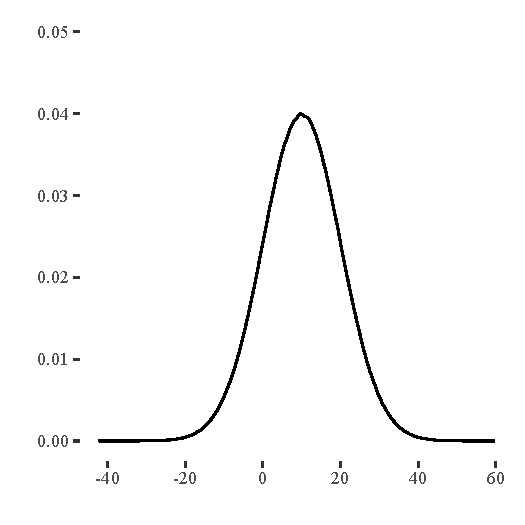
\includegraphics{AdditivityOfVariance_files/figure-latex/unnamed-chunk-8-1} 

}

\caption[$N(\mu_d, \sigma^2_d)$の分布]{$N(\mu_d, \sigma^2_d)$の分布}\label{fig:unnamed-chunk-8}
\end{marginfigure}

\begin{marginfigure}

{\centering 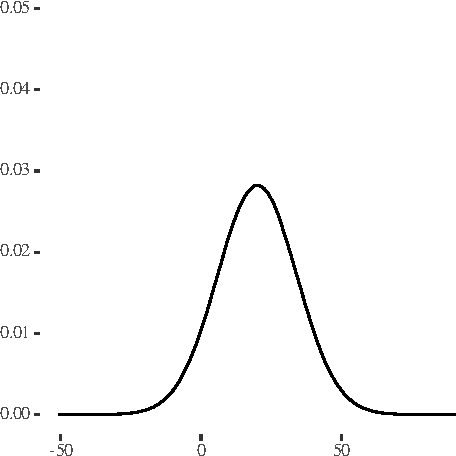
\includegraphics{AdditivityOfVariance_files/figure-latex/unnamed-chunk-9-1} 

}

\caption[$N(\mu_e, \sigma^2_e)$の分布]{$N(\mu_e, \sigma^2_e)$の分布}\label{fig:unnamed-chunk-9}
\end{marginfigure}

\newpage

\hypertarget{ux540cux4e00ux306eux6b63ux898fux5206ux5e03ux304bux3089ux53d6ux308aux51faux3057ux305fux5024ux3092ux5e73ux5747ux3057ux305fux5834ux5408}{%
\subsection{\texorpdfstring{\textbf{同一の正規分布から取り出した値を平均した場合}}{同一の正規分布から取り出した値を平均した場合}}\label{ux540cux4e00ux306eux6b63ux898fux5206ux5e03ux304bux3089ux53d6ux308aux51faux3057ux305fux5024ux3092ux5e73ux5747ux3057ux305fux5834ux5408}}

 最後に同一の正規分布\(N(\mu_d, \sigma^2_d)\)から取り出した二つの値の\textbf{平均値の分布}を考えてみます。「二つの値の平均値の平均値」とは、正規分布\(N(\mu_d, \sigma^2_d)\)から、ランダムサンプリングで二つの値を取り出して、その平均値を取るということです。取り出した値は元の正規分布へ戻し、同様の操作を繰り返します。

\begin{Shaded}
\begin{Highlighting}[numbers=left,,]
\NormalTok{f }\OtherTok{\textless{}{-}} \FunctionTok{c}\NormalTok{((}\FunctionTok{sample}\NormalTok{(d, n, }\AttributeTok{replace =} \ConstantTok{TRUE}\NormalTok{) }\SpecialCharTok{+} \FunctionTok{sample}\NormalTok{(d, n, }\AttributeTok{replace =} \ConstantTok{TRUE}\NormalTok{)) }\SpecialCharTok{/} \DecValTok{2}\NormalTok{)}
\FunctionTok{head}\NormalTok{(f, }\DecValTok{20}\NormalTok{)}
\end{Highlighting}
\end{Shaded}

\begin{verbatim}
##  [1]  8.7305884 14.9020097  8.8849919 16.4786882  8.3310684  5.1886257
##  [7] 12.4705646 -1.5500875 -0.5659579  9.1376441 11.6390996 18.5703466
## [13]  9.7226476 15.8533947 19.5455885 11.9792291 11.4669204  3.8360299
## [19] 15.0274205 16.0350309
\end{verbatim}

この正規分布正規分布\(N(\mu_f, \sigma^2_f)\)は、二つの値の平均値、つまり二つの値を半分に割った値ですので正規分布\(N(2\mu_d, 2\sigma^2_d)\)のすべての値を半分にした正規分布になると予想できます。

\[\mbox{「二つの標本の平均値」の平均値} = \frac{2\mu_d}{2} = \mu_d\]

\[\mbox{「二つの標本の平均値」の標準偏差} = \sqrt{\frac{2\sigma^2_d}{2}} = \frac{\sigma_d}{\sqrt{2}}\]

\[\mbox{「二つの標本の平均値」の分散} = (\frac{\sigma_d}{\sqrt{2}})^2 = \frac{\sigma^2_d}{2}\]

\begin{marginfigure}

{\centering 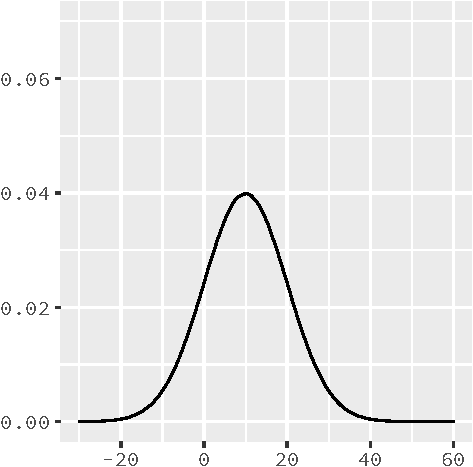
\includegraphics{AdditivityOfVariance_files/figure-latex/unnamed-chunk-11-1} 

}

\caption[$N(\mu_d, \sigma^2_d)$の分布]{$N(\mu_d, \sigma^2_d)$の分布}\label{fig:unnamed-chunk-11}
\end{marginfigure}

\begin{marginfigure}

{\centering 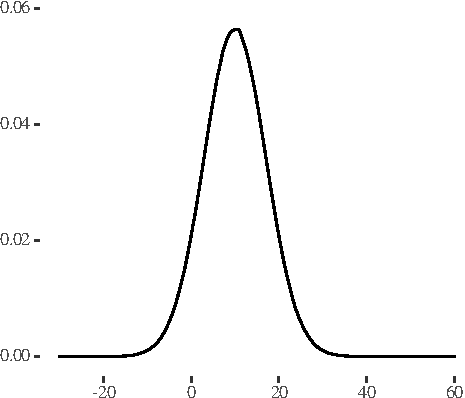
\includegraphics{AdditivityOfVariance_files/figure-latex/unnamed-chunk-12-1} 

}

\caption[$N(\mu_f, \sigma^2_f)$の分布]{$N(\mu_f, \sigma^2_f)$の分布}\label{fig:unnamed-chunk-12}
\end{marginfigure}

\begin{longtable}[]{@{}lcccl@{}}
\toprule
正規分布 & 平均 & 分散 & 標準偏差 & 備考 \\
\midrule
\endhead
\(N(\mu_d, \sigma^2_d)\) & 10.0026499 & 99.9740994 & 9.9987049 &
元の分布 \\
\(N(\mu_d, \frac{\sigma^2_d)}{2}\) & 10.0026499 & 49.9870497 & 7.070152
& 分散の加法性 \\
\(N(\mu_f, \sigma^2_f)\) & 10.0038582 & 49.9996318 & 7.0710418 & \\
\bottomrule
\end{longtable}

このように元の分布よりも鋭い分布になっていることがわかります。

\newpage

\hypertarget{about-handout-style}{%
\section{\texorpdfstring{\textbf{About handout
style}}{About handout style}}\label{about-handout-style}}

The Tufte handout style is a style that Edward Tufte uses in his books
and handouts. Tufte's style is known for its extensive use of sidenotes,
tight integration of graphics with text, and well-set typography. This
style has been implemented in LaTeX and HTML/CSS\footnote{See Github
  repositories
  \href{https://github.com/tufte-latex/tufte-latex}{tufte-latex} and
  \href{https://github.com/edwardtufte/tufte-css}{tufte-css}},
respectively.

 

\bibliography{bib/references.bib}



\end{document}
